\chapter{Lookahead}
\label{ch:epilogue}


 When you consider that the cryptocurrency market remains highly volatile and largely unregulated, it is still highly speculative to invest in any of it. The road to mass adoption is not without significant hiccups. We need to give distribute ledger technology and blockchain technology time to mature. If given that time, all these daring and promising startups will have to prove themselves, just like any other company and any other technology. Even though there is much debate around the question how we should deal with blockchain and cryptocurrencies in the coming years.

       \bigskip 
       \begin{quotation}
              \textit{\say{While technological change has been incredibly fast in the information era, the system of international payments has lagged.}}
              \begin{flushright}
                \small{--- \textbf{Don Tapscott}}
              \end{flushright}
        \end{quotation}   
  

\begin{figure}
\centering
    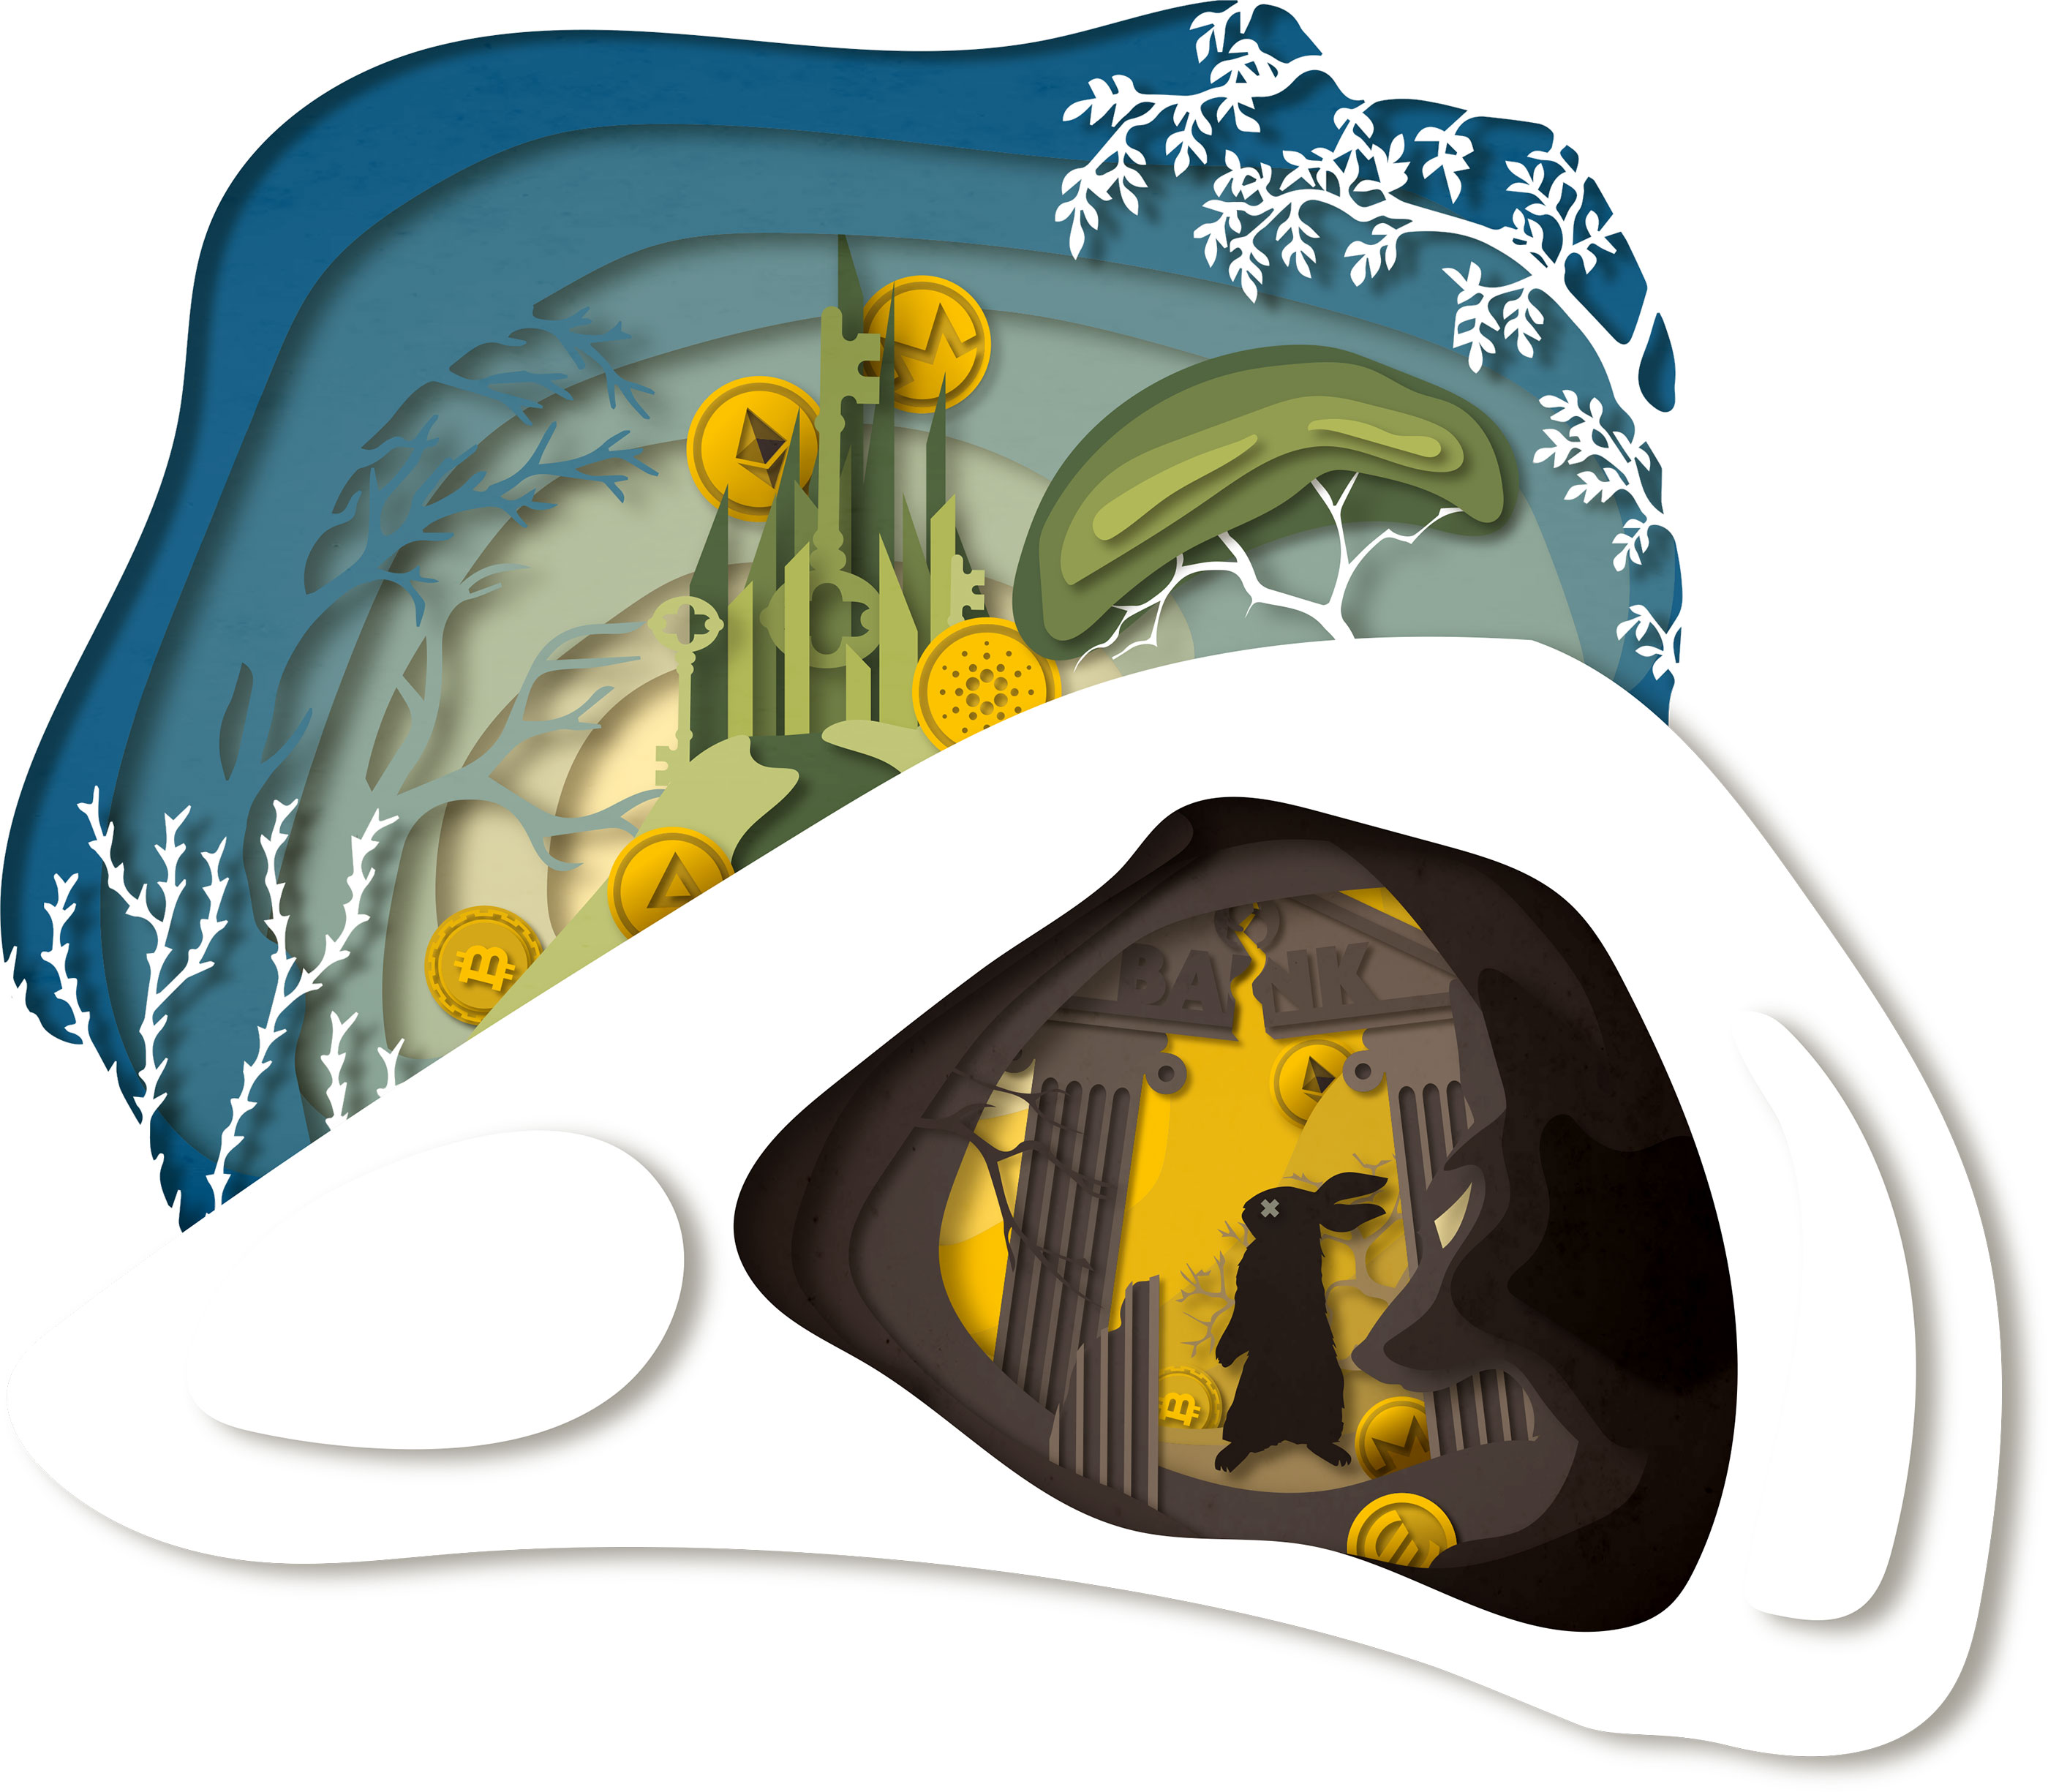
\includegraphics[width=\textwidth]{illustrations/resized_CRYPTO_KEY_1_PART_2.jpg}
\end{figure}

\section*{Financial-technology sector}
This market has enormous potential when you think of the possibilities for potential growth on investments in the long term since it is still in its infancy stages. Some of these projects are here to stay, and many more are starting every day, introducing healthy competition that is going to boost the fin-tech industry. There is an ever-increasing demand for skilled people in the fin-tech sector. Businesses cannot seem to find enough software engineers and blockchain developers, and everyone can get into it - take several free courses available on the internet to get you up to speed and develop new skill-sets that might boost your career and give you a new direction - this industry is just getting started. Not to mention the fact that the younger generations have been growing up in the digital age and the impact this makes on their lives cannot be unseen.

\section*{Open and decentralized finance}
Cryptocurrencies, particularly Bitcoin, already have massive momentum. We are not predicting whether or not all of this will eventually succeed. However, we do believe that the economy works best when it works for everyone, and this new platform represents an engine which stimulates and enables inclusion. Open blockchain significantly lowers the requirements for people to obtain access to financial services and will compete with traditional central banking models.

    \bigskip
    \begin{cryptobox}{\textbf{MONEY AT THE BANK}}
        In summary, when you store money at the bank - and in the possible future at corporations - the bank becomes the owner of that money. With Bitcoin, \emph{you} own your money. When the banks own that money, they spend it as they wish. When you own it, \emph{you} spend it as you wish. It is censorship-resistant, and no one decides on what you can or cannot spend it.
    \end{cryptobox}

\section*{New Regulations}
Blockchain will be an integral element in our future infrastructures. The challenge is to oversee and guide the adoption process. Even though it may sound bad for cryptocurrency or blockchain in general - as long as its stimulates innovation - adaptive governments and nimble and experimental regulation, legislation and compliance policies will be of crucial importance to propel development forward. 


\section*{Disrupting industries}
Besides Bitcoin, there are hundreds of other projects out there that are working on solving some of the most pressing matters in our financial spheres and other industries like supply chain, healthcare, energy and content creation. Mainly, the success of blockchain technology has already been set in stone since it's not dependent on cryptocurrency alone. Where blockchain can serve as a decentralised ledger that securely stores immutable data, we can also use it as such without the use of any cryptocurrencies. Cryptocurrencies or tokens might be used on specific networks because they have a serve a particular function. They might function as a utility token or as a means of payment to the network or to store, capture or move value around in the form of a digital currency.\medskip

\section*{Both the economy and currencies need to evolve}

In terms of global macroeconomic developments, and after having taken a more in-depth look at the blockchain and cryptocurrency spheres, we note many indicators which lead us to believe that rapid, drastic change may lie around the corner. We actively research these areas and look at these global developments, which are driving innovation and change. We see trends that have the potential to radically change vast chunks of industry and change the lives of billions of people and find hope and opportunity in areas where others may not. In the face of any crisis, there is \emph{always} ample room for new growth, in directions that may come as a surprise to many. What will happen when the inevitable strikes? Will economies collapse globally? Will life as we know it, be a thing of the past? If history is any indication, governments and banks will, once again, try to change the rules. 

    \begin{quotation}
        \textit{\say{In the midst of every crisis, lies great opportunity.}}
            \begin{flushright}
                \small{--- \textbf{Albert Einstein}}
            \end{flushright}
    \end{quotation}

\section*{New Economy}
We believe that this transition heralds the beginning of a new economic era, of an inclusive economy, where people's (intellectual) contributions are valued and rewarded according to the added value they bring to the economy as a whole, their immediate environment, community or family and friends. With Cryptomanuals, we inform people of what is going on in the global economy, provide some historical context and point out one of the most significant opportunities and wealth transfers of our lifetimes. 


    \bigskip
    \begin{cryptobox}{\textbf{SUGGESTIONS}}
        Don't forget to check out our pre-selection of useful applications, tools, videos and other information.
        \tcblower
        You can start right away on our website:
        \begin{enumerate}
            \setlength\itemsep{0em}
            \item With the \href{https://cryptomanuals.com/start-with-cryptocurrency/}{five steps to start}.
            \item There are many ways to earn   \href{https://cryptomanuals.com/free-cryptomanuals/}{free crypto}.
            \item A pre-selection of useful \href{https://cryptomanuals.com/5-tools-to-buy-trade-and-manage-your-crypto-portfolio/}{portfolio tools}.
            \item Take a look at our selected  \href{https://cryptomanuals.com/5-videos-to-start-with-bitcoin/}{Bitcoin videos}.
            \item A selection of  \href{https://cryptomanuals.com/5-applications-to-enhance-online-privacy-and-security/}{privacy tools}.
        \end{enumerate}
    \end{cryptobox}